\section{Input data definition}
\subsection{Exposure model definition}
All risk calculators in the OpenQuake engine require an \gls{exposure model} that needs to be stored in NRML. There are a number of parameters that compose the metadata, and provides general information regarding the \glspl{asset} within the \gls{exposure model}, as described below:

\begin{itemize}
\item  \Verb+id+: a unique key used to identify the \gls{exposure model};
\item  \Verb+category+: a string used to define the type of \glspl{asset} being stored (e.g: buildings, population, contents);
\item  \Verb+taxonomySource+: attribute used to define the \gls{taxonomy} being used to classify the  \glspl{asset};
\item  \Verb+description+: brief string with further information about the \gls{exposure model};
\end{itemize}

This information is common to all the assets and needs to be incorporated at the beginning of the exposure model file according to the following example:

\begin{Verbatim}[frame=single, commandchars=\\\{\}, samepage=false]
<?xml version="1.0" encoding="UTF-8"?>
<nrml xmlns="http://openquake.org/xmlns/nrml/0.4">
<\textcolor{red}{exposureModel} id="ex1"
      category="buildings"
      taxonomySource="GEM taxonomy">
    <\textcolor{green}{description}> Buildings in Pavia </\textcolor{green}{description}>
...
\end{Verbatim}

The NRML schema for the exposure model allows the definition of various types of costs (structural cost, nonstructural cost, contents cost, business interruption cost). Further explanations regarding the quantities that are currently being used to define the exposure elements can be found in the OpenQuake Engine Book (Risk).
\\
The way the information about the characteristics of the \glspl{asset} in an \gls{exposure model} are stored can vary strongly depending on how and why the data was compiled. As an example, if national census information is used to estimated the distribution of assets in a given region, it is likely that the number of buildings within a given geographical area will be used to define the dataset, and will be used for estimating the number of collapsed buildings for a scenario earthquake. On the other hand, if simplified methodologies based on proxy data such as population distribution are used to develop the exposure model, then it is likely that the built up area or economic cost of each building typology will be directly derived, and will be used for the estimation of economic losses. Thus, the following set of attributes exist within the schema for the exposure model:

\begin{itemize}
\item  \Verb+number+: number of units of a given \gls{asset} at a given location;
\item  \Verb+area+: area of the \gls{asset}, at a given location;
\item  \Verb+cost+: structural replacement cost of the \gls{asset} at a given location;
\end{itemize}

The set of required attributes depends on what and how a user wants to store the information about the assets in the exposure model. While the attribute \Verb+number+ might be a rather simple parameter, the other two (area and cost) can be ambiguous, as different ways to define them might be used. With regards to the attribute \Verb+area+, one can either choose to provide the aggregated built up area of the \glspl{asset} per location or the average built up area for a single building unit (noting that an \gls{asset} might be made up of a number of individual buildings). Similarly, the \Verb+cost+ can also be defined as the aggregated structural replacement cost, the cost of replacing a single unit or even the structural replacement cost per unit of area. For the purposes of performing a retrofitting benefit/cost analysis, it is also necessary to define the retrofitting cost (\Verb+reco+). The combination between the possible options in which these three attributes can be defined leads to four ways of storing the information about the assets. For each of these cases a brief explanation and example is provided in this section.

\paragraph{Example 1}
This example is comprised of an \gls{exposure model} in which the aggregated cost (structural, nonstructural, contents and business interruption) of the buildings of each taxonomy for a set of locations is directly provided. Thus, in order to indicate how the various costs will be defined, the following information needs to be stored in the exposure model file:

\begin{Verbatim}[frame=single, commandchars=\\\{\}, samepage=false]
...
 <\textcolor{green}{conversions}>
  <\textcolor{blue}{costTypes}>
   <\textcolor{magenta}{costType} name="structural" type="aggregated" unit="EUR">
   <\textcolor{magenta}{costType} name="non_structural" type="aggregated" unit="EUR" />
   <\textcolor{magenta}{costType} name="business_interruption" type="aggregated" 
                                                      unit="EUR"/>
   <\textcolor{magenta}{costType} name="contents" type="aggregated" unit="EUR"/>
  </\textcolor{blue}{costTypes}>
 </\textcolor{green}{conversions}>
...
\end{Verbatim}

In this case, the cost \Verb+type+ of each component as been defined as \Verb+aggregated+. Once the way in which each cost is going to be defined has been established, the values for each asset can be stored according to the following format.

\begin{Verbatim}[frame=single, commandchars=\\\{\}, samepage=false]
...
 <\textcolor{green}{assets}>
  <\textcolor{blue}{asset} id="asset_01" taxonomy="RC/DMRF-D/LR">
   <\textcolor{magenta}{location} lon="9.15" lat="45.17" />
   <\textcolor{magenta}{costs}>
    <cost type="structural" value="1500"/>
    <cost type="non_structural" value="2500"/>
    <cost type="contents" value="1200"/>
    <cost type="business_interruption" value="400"/>
   </\textcolor{magenta}{costs}>
  </\textcolor{blue}{asset}>
...
  <\textcolor{blue}{asset} id="asset_99"  taxonomy="RC/DMRF-D/HR">
   <\textcolor{magenta}{location} lon="9.15" lat="45.12" />
   <\textcolor{magenta}{costs}>
    <cost type="structural" value="2500"/>
    <cost type="non_structural" value="2100"/>
    <cost type="contents" value="1900"/>
    <cost type="business_interruption" value="40"/>
   </\textcolor{magenta}{costs}>
  </\textcolor{blue}{asset}>
 </\textcolor{green}{assets}>
</\textcolor{red}{exposureModel}>
</nrml>
\end{Verbatim}

Each \gls{asset} is uniquely identified by its \Verb+id+, which is used by the OpenQuake engine to relate each asset with the associated results (e.g. loss exceedance curves). Then, a pair of coordinates (latitude and longitude) for a \Verb+location+ where the asset is assumed to exist is defined. Each asset must be classified according to a \Verb+taxonomy+, so that the OpenQuake engine is capable of employing the appropriate \gls{vulnerability function} or \gls{fragility function} in the risk calculations. Finally, the cost values of each \Verb+type+ are stored within the \Verb+costs+ attribute. In this example, the aggregated value for all units (within a given asset) at each location is provided directly, so there is no need to define other attributes such as \Verb+number+ or \Verb+area+. This mode of representing an exposure model is probably the simplest one.

\paragraph{Example 2}
In this example an \gls{exposure model} containing the number of units (buildings) and the associated costs per unit of each building typology is presented.

\begin{Verbatim}[frame=single, commandchars=\\\{\}, samepage=false]
...
 <\textcolor{green}{conversions}>
  <\textcolor{blue}{costTypes}>
   <\textcolor{magenta}{costType} name="structural" type="per_unit" unit="EUR">
   <\textcolor{magenta}{costType} name="non_structural" type="per_unit" unit="EUR" />
   <\textcolor{magenta}{costType} name="business_interruption" type="per_unit" 
                                                      unit="EUR"/>
   <\textcolor{magenta}{costType} name="contents" type="per_unit" unit="EUR"/>
  </\textcolor{blue}{costTypes}>
 </\textcolor{green}{conversions}>
...
\end{Verbatim}

For this case, the cost \Verb+type+ has been set to \Verb+per_unit+. Then, the information from each asset can be stored following the format below.  

\begin{Verbatim}[frame=single, commandchars=\\\{\}, samepage=false]
...
 <\textcolor{green}{assets}>
  <\textcolor{blue}{asset} id="asset_01" number="10" taxonomy="RC/DMRF-D/LR">
   <\textcolor{magenta}{location} lon="9.15" lat="45.17" />
   <\textcolor{magenta}{costs}>
    <cost type="structural" value="150"/>
    <cost type="non_structural" value="250"/>
    <cost type="contents" value="120"/>
    <cost type="business_interruption" value="40"/>
   </\textcolor{magenta}{costs}>
  </\textcolor{blue}{asset}>
...
  <\textcolor{blue}{asset} id="asset_99" number="20" taxonomy="RC/DMRF-D/HR">
   <\textcolor{magenta}{location} lon="9.15" lat="45.12" />
   <\textcolor{magenta}{costs}>
    <cost type="structural" value="125"/>
    <cost type="non_structural" value="105"/>
    <cost type="contents" value="95"/>
    <cost type="business_interruption" value="20"/>
   </\textcolor{magenta}{costs}>
  </\textcolor{blue}{asset}>
 </\textcolor{green}{assets}>
</\textcolor{red}{exposureModel}>
</nrml>
\end{Verbatim}

In this example, the various costs for each asset is not provided directly, as happened in the previous example. In order to carry out the risk calculations in which the economic cost of each asset is required, the OpenQuake engine multiplies, for each asset, the number of units (buildings) by the "per unit" replacement cost. Note that in this case, there is no need to specify the attribute \Verb+area+. 

\paragraph{Example 3}
This example is comprised of an \gls{exposure model} containing the built up area of each building typology for a set of locations, and the associated costs per area.

\begin{Verbatim}[frame=single, commandchars=\\\{\}, samepage=false]
...
 <\textcolor{green}{conversions}>
  <\textcolor{blue}{area} type="aggregated" unit="square meters"/>
  <\textcolor{blue}{costTypes}>
   <\textcolor{magenta}{costType} name="structural" type="per_area" unit="EUR">
   <\textcolor{magenta}{costType} name="non_structural" type="per_area" unit="EUR" />
   <\textcolor{magenta}{costType} name="business_interruption" type="per_area" 
                                                      unit="EUR"/>
   <\textcolor{magenta}{costType} name="contents" type="per_area" unit="EUR"/>
  </\textcolor{blue}{costTypes}>
 </\textcolor{green}{conversions}>
...
\end{Verbatim}

In order to compile an \gls{exposure model} with this structure, it is required to set the cost \Verb+type+ to \Verb+per_area+. In addition, it is also necessary to specify if the \Verb+area+ that is being store represents the aggregated area of number of units within an asset, or the average area of a single unit. In this particular case, the \Verb+area+ that is being stored is the aggregated built up area per asset, and thus this attribute was set to \Verb+aggregated+.  

\begin{Verbatim}[frame=single, commandchars=\\\{\}, samepage=false]
...
 <\textcolor{green}{assets}>
  <\textcolor{blue}{asset} id="asset_01" area="50" taxonomy="RC/DMRF-D/LR">
   <\textcolor{magenta}{location} lon="9.15" lat="45.17" />
   <\textcolor{magenta}{costs}>
    <cost type="structural" value="100"/>
    <cost type="non_structural" value="200"/>
    <cost type="contents" value="90"/>
    <cost type="business_interruption" value="10"/>
   </\textcolor{magenta}{costs}>
  </\textcolor{blue}{asset}>
...
  <\textcolor{blue}{asset} id="asset_99" area ="60" taxonomy="RC/DMRF-D/HR">
   <\textcolor{magenta}{location} lon="9.15" lat="45.12" />
   <\textcolor{magenta}{costs}>
    <cost type="structural" value="150"/>
    <cost type="non_structural" value="250"/>
    <cost type="contents" value="50"/>
    <cost type="business_interruption" value="30"/>
   </\textcolor{magenta}{costs}>
  </\textcolor{blue}{asset}>
 </\textcolor{green}{assets}>
</\textcolor{red}{exposureModel}>
</nrml>
\end{Verbatim}

Once again, the OpenQuake engine needs to carry out some calculations in order to compute the different costs per asset. In this case, this value is computed by multiplying the aggregated built up \Verb+area+ of each building typology by the associated cost per unit of area. Notice that in this case, there is no need to specify the attribute \Verb+number+.

\paragraph{Example 4}
This example is comprised of an \gls{exposure model} containing the number of buildings for each location, the average built up area per building unit and the associated costs per area. 

\begin{Verbatim}[frame=single, commandchars=\\\{\}, samepage=false]
...
 <\textcolor{green}{conversions}>
  <\textcolor{blue}{area} type="per_asset" unit="square meters"/>
  <\textcolor{blue}{costTypes}>
   <\textcolor{magenta}{costType} name="structural" type="per_area" unit="EUR">
   <\textcolor{magenta}{costType} name="non_structural" type="per_area" unit="EUR" />
   <\textcolor{magenta}{costType} name="business_interruption" type="per_area" 
                                                      unit="EUR"/>
   <\textcolor{magenta}{costType} name="contents" type="per_area" unit="EUR"/>
  </\textcolor{blue}{costTypes}>
 </\textcolor{green}{conversions}>
...
\end{Verbatim}

Similarly to what was described in the previous example, the various costs \Verb+type+ also need to be establish as \Verb+per_area+, but the \Verb+type+ of area is now defined as \Verb+per_unit+.

\begin{Verbatim}[frame=single, commandchars=\\\{\}, samepage=false]
...
 <\textcolor{green}{assets}>
  <\textcolor{blue}{asset} id="asset_01" number="5" area="50" taxonomy="RC/DMRF-D/LR">
   <\textcolor{magenta}{location} lon="9.15" lat="45.17" />
   <\textcolor{magenta}{costs}>
    <cost type="structural" value="100"/>
    <cost type="non_structural" value="200"/>
    <cost type="contents" value="90"/>
    <cost type="business_interruption" value="10"/>
   </\textcolor{magenta}{costs}>
  </\textcolor{blue}{asset}>
...
  <\textcolor{blue}{asset} id="asset_99" number="8" area ="60" taxonomy="RC/DMRF-D/HR">
   <\textcolor{magenta}{location} lon="9.15" lat="45.12" />
   <\textcolor{magenta}{costs}>
    <cost type="structural" value="150"/>
    <cost type="non_structural" value="250"/>
    <cost type="contents" value="50"/>
    <cost type="business_interruption" value="30"/>
   </\textcolor{magenta}{costs}>
  </\textcolor{blue}{asset}>
 </\textcolor{green}{assets}>
</\textcolor{red}{exposureModel}>
</nrml>
\end{Verbatim}

In this example, the OpenQuake engine will make use of all the parameters to estimate the various costs of each asset, by multiplying the number of buildings by its average built up area, and then by the respective cost per unit of area. 

\paragraph{Example 5}
In this example, additional information will be included, which is required for other risk analysis besides loss estimation, such as the calculation of insured losses or benefit/cost analysis. For the former assessment, it is necessary to establish how the insured limit and deductible is going to be define, according to the format below. 
\begin{Verbatim}[frame=single, commandchars=\\\{\}, samepage=false]
...
 <\textcolor{green}{conversions}>
  <\textcolor{blue}{costTypes}>
   <\textcolor{magenta}{costType} name="structural" type="aggregated" unit="EUR">
   <\textcolor{magenta}{costType} name="non_structural" type="aggregated" unit="EUR" />
   <\textcolor{magenta}{costType} name="business_interruption" type="aggregated" 
                                                      unit="EUR"/>
   <\textcolor{magenta}{costType} name="contents" type="aggregated" unit="EUR"/>
  </\textcolor{blue}{costTypes}>
  <\textcolor{blue}{deductible} isAbsolute="false"/>
  <\textcolor{blue}{insuranceLimit} isAbsolute="false"/>
 </\textcolor{green}{conversions}>
...
\end{Verbatim}

In this example, both the insurance limit and the deductible were defined as a fraction of the costs, by setting the attribute \Verb+isAbsolute+ to \Verb+false+. On the other hand, a user could define one or both of these parameters as the absolute threshold, by setting the aforementioned attribute to \Verb+true+. Then, for each type of cost, the limit and deductible value can be stored for each asset.
Moreover, in order to perform a benefit/cost assessment, it is also fundamental to indicate the retrofitting cost. This parameter is handled in the same manner as the structural cost, and it should be stored according to the following structure. 

\begin{Verbatim}[frame=single, commandchars=\\\{\}, samepage=false]
...
 <\textcolor{green}{assets}>
  <\textcolor{blue}{asset} id="asset_01" taxonomy="RC/DMRF-D/LR">
   <\textcolor{magenta}{location} lon="9.15" lat="45.17" />
   <\textcolor{magenta}{costs}>
    <cost type="structural" value="1500" deductible=".05" 
                insuranceLimit="0.9" retrofitted="200"/>
    <cost type="non_structural" value="2500" deductible=".1" 
                insuranceLimit="0.8"/>
    <cost type="contents" value="1200" deductible=".2" 
                insuranceLimit="0.6"/>
    <cost type="business_interruption" value="400" deductible=".1" 
                insuranceLimit="0.5"/>
   </\textcolor{magenta}{costs}>
  </\textcolor{blue}{asset}>
...
  <\textcolor{blue}{asset} id="asset_99"  taxonomy="RC/DMRF-D/HR">
   <\textcolor{magenta}{location} lon="9.15" lat="45.12" />
   <\textcolor{magenta}{costs}>
    <cost type="structural" value="2500" deductible=".1" 
                insuranceLimit="0.9"/ retrofitted="300"/>
    <cost type="non_structural" value="2100" deductible=".05" 
                insuranceLimit="0.7"/>
    <cost type="contents" value="1900" deductible=".2" 
                insuranceLimit="0.7"/>
    <cost type="business_interruption" value="40"/ deductible=".05" 
                insuranceLimit="0.9">
   </\textcolor{magenta}{costs}>
  </\textcolor{blue}{asset}>
 </\textcolor{green}{assets}>
</\textcolor{red}{exposureModel}>
</nrml>
\end{Verbatim}

Despite the fact that for the demonstration of how the insurance parameters and retrofitting cost can be stored it was used the aggregated type of cost (structure described in example 1), it is important to mention that any of the other storing approaches can also be employed (example 2 -4).

\paragraph{Example 6}
The OpenQuake engine is also capable of estimating human losses, based on a number of occupants within an asset, at a certain time of the day. In this example, it is demonstrated how this parameter is defined for each asset. In addition, this example also serves the purpose of presenting an \gls{exposure model} in which three cost types have been defined following different structures.

\begin{Verbatim}[frame=single, commandchars=\\\{\}, samepage=false]
...
 <\textcolor{green}{conversions}>
  <\textcolor{blue}{area} type="aggregated" unit="square meters"/>
  <\textcolor{blue}{costTypes}>
   <\textcolor{magenta}{costType} name="structural" type="per_unit" unit="EUR">
   <\textcolor{magenta}{costType} name="non_structural" type="per_area" unit="EUR" />
   <\textcolor{magenta}{costType} name="contents" type="aggregated" unit="EUR"/>
  </\textcolor{blue}{costTypes}>
 </\textcolor{green}{conversions}>
...
\end{Verbatim}

As previously mentioned, in this example only three costs are being stored, and each one follows a different approach. The \Verb+structural+ cost is being defined as the replacement cost per unit (example 2), the \Verb+non_structural+ cost is established as the cost per area (example 3), and the \Verb+contents+ cost is provided directly as the aggregated value per asset (example 1). The information about each asset is presented bellow, along with the number of occupants at different times of the day.

\begin{Verbatim}[frame=single, commandchars=\\\{\}, samepage=false]
...
 <\textcolor{green}{assets}>
  <\textcolor{blue}{asset} id="asset_01" number="5" area ="500" taxonomy="RC/DMRF-D/LR">
   <\textcolor{magenta}{location} lon="9.15" lat="45.17" />
   <\textcolor{magenta}{costs}>
    <cost type="structural" value="1000"/>
    <cost type="non_structural" value="250"/>
    <cost type="contents" value="5000"/>
   </\textcolor{magenta}{costs}>
   <\textcolor{magenta}{occupancies}>
    <occupancy occupants="10" period="day"/>
    <occupancy occupants="50" period="night"/>
   </\textcolor{magenta}{occupancies}>
  </\textcolor{blue}{asset}>
...
  <\textcolor{blue}{asset} id="asset_99" number="8" area ="800" taxonomy="RC/DMRF-D/HR">
   <\textcolor{magenta}{location} lon="9.15" lat="45.12" />
   <\textcolor{magenta}{costs}>
    <cost type="structural" value="2000"/>
    <cost type="non_structural" value="400"/>
    <cost type="contents" value="4000"/>
   </\textcolor{magenta}{costs}>
   <\textcolor{magenta}{occupancies}>
    <occupancy occupants="20" period="day"/>
    <occupancy occupants="30" period="night"/>
   </\textcolor{magenta}{occupancies}>
  </\textcolor{blue}{asset}>
 </\textcolor{green}{assets}>
</\textcolor{red}{exposureModel}>
</nrml>
\end{Verbatim}

The number of occupants for each asset is stored under the \Verb+occupancies+ field, as part of the \Verb+occupancy+ instance. The number and type of periods of the day is not a fixed variable, and a user can provide as many as needed (e.g. morning, afternoon, night, transit, 9am-17pm). The descriptions used to define each \Verb+period+ are used to specify the time of the day for which the human losses should be estimated in the Scenario Risk calculator (see section INCLUDE LATER).

The way this information is being stored is constantly being modified, as further feedback from users and experts is received. Hence, it is important to understand which version of NRML the engine is using, in order to avoid incompatibility issues. NRML is currenly v0.4 and documentation about each release can be found on GitHub (see \href{http://gitub.com/gem/oq-nrmllib}{oq-nrmllib}). Several examples of \glspl{exposure model} containing different types of information are presented below. 

\subsection{Physical vulnerability model definition}
In this section, the NRML schema for the \gls{vulnerability model} is described in detail. In order to do so, a graphical representation of a \gls{vulnerability model} (mean loss ratio for a set of intensity measure levels) is illustrated in Figure \ref{fig:vulModel}, and the equivalent NRML file is then presented. Note that although the uncertainty for each loss ratio is not represented in the aforementioned figure, it has been considered in the input NRML file, by means of a coefficient of variation per loss ratio and a probabilistic distribution, which can currently be set to lognormal or beta. This model is comprised of two discrete \glspl{vulnerability function} and uses spectral acceleration for a given period of vibration as the intensity measure type. 

\begin{figure}[ht]
\centering
\includegraphics[width=10cm,height=6cm]{./figures/risk/vulnerabilityModel.pdf}
\caption{Graphical representation of a vulnerability model.}
\label{fig:vulModel}
\end{figure}

Each component of the associated NRML file is presented herein:
 
\begin{Verbatim}[frame=single, commandchars=\\\{\}, samepage=true]
<?xml version="1.0" encoding="UTF-8"?>
<nrml xmlns:gml="http://www.opengis.net/gml"
      xmlns="http://openquake.org/xmlns/nrml/0.4">
<\textcolor{red}{vulnerabilityModel}>
    <\textcolor{green}{discreteVulnerabilitySet} vulnerabilitySetID="OpenQuake2013"	
    assetCategory="buildings"    lossCategory="economic loss">
        ...
\end{Verbatim}

At the top of the NRML schema, the following metadata are being stored:
\begin{itemize}
\item  \Verb+vulnerabilitySetID+: A unique key used to identify the \gls{vulnerability model} instance within the OpenQuake engine;
\item  \Verb+assetCategory+: An attribute that describes the asset typology (e.g.: population, buildings, contents);
\item  \Verb+lossCategory+: An attribute that describes the type of loss being modelled for the assetCategory (e.g. fatalities, structural replacement cost, contents replacement cost). 
\end{itemize}

\begin{Verbatim}[frame=single, commandchars=\\\{\}, samepage=true]
    ...
        <\textcolor{blue}{IML}  IMT = "SA(0.3)"> 0.061 0.129 0.188 0.273 0.398 0.579 
        0.843 1.227 1.856 2.485 <\textcolor{blue}{/IML}>
        ...
\end{Verbatim}

Within this component, an attribute specifying the intensity measure type (e.g.: Sa, PGA, MMI) is defined, followed by the list of intensity measure levels. This set of values is common to all of the \glspl{vulnerability function} in the model.

\begin{Verbatim}[frame=single, commandchars=\\\{\}, samepage=true]
        ...
        <\textcolor{blue}{discreteVulnerability}  vulnerabilityFunctionID="typeA" 
        probabilisticDistribution="LN">
            <\textcolor{magenta}{lossRatio}> 0.002 0.007 0.014 0.028 0.058 0.118
            0.223 0.370 0.446 0.523 <\textcolor{magenta}{/lossRatio}>
            <\textcolor{magenta}{coefficientsVariation}> 0.012 0.058 0.079 0.159 0.265 
            0.244 0.211 0.152 0.088 0.082 <\textcolor{magenta}{/coefficientsVariation}>
        <\textcolor{blue}{/discreteVulnerability}>
        <\textcolor{blue}{discreteVulnerability}  vulnerabilityFunctionID="typeB" 
        probabilisticDistribution="LN">
            <\textcolor{magenta}{lossRatio}> 0.006 0.025 0.052 0.108 0.215 0.391	
            0.613 0.820 0.894 0.967 <\textcolor{magenta}{/lossRatio}>
            <\textcolor{magenta}{coefficientsVariation}> 0.010 0.054 0.082 0.167 0.285 
            0.278 0.261 0.132 0.084 0.021 <\textcolor{magenta}{/coefficientsVariation}>
        <\textcolor{blue}{/discreteVulnerability}>
    <\textcolor{green}{/discreteVulnerabilitySet} 
<\textcolor{red}{/vulnerabilityModel}>        
</nrml>
\end{Verbatim}

Finally, for each discrete \gls{vulnerability function} the following parameters are required:
\begin{itemize}
\item  \Verb+ vulnerabilityFunctionID +: A unique key that is used to relate each \gls{vulnerability function} with the \glspl{asset} in the \gls{exposure model};
\item  \Verb+ probabilisticDistribution +: An attribute that establishes the type of probabilistic distribution used to model the uncertainty in loss ratio. At the moment, the OpenQuake engine supports lognormal (\Verb+LN+) and beta (\Verb+BT+) distributions;
\item  \Verb+ lossRatio +: A set of mean loss ratios (one for each intensity measure level defined previously). These values can represent different losses such as fatality rates (ratio between the number of fatalities and total population exposed) or so-called damage ratio (ratio between the repair cost and the replacement cost of a given structure).
\item  \Verb+ coefficientsVariation +: A set of coefficients of variation (one per loss ratio) that describes the uncertainty in the loss ratio. If users do not want to consider the uncertainty, this set of parameters can be set to zero, and the OpenQuake engine assumes each loss ratio as a deterministic value. 
\end{itemize}

In the previously described \gls{vulnerability model} all of the \glspl{vulnerability function} were defined in terms of a single intensity measure type (Sa for 0.3 seconds). However, the current version of the engine also allows the employment of a \gls{vulnerability model} that is comprised of \glspl{vulnerability function} that each use distinct intensity measure types. In the following example, the schema of a \gls{vulnerability model} in which three intensity measure types were used (PGA, PGV and Sa for 0.3 seconds) is presented.

\begin{Verbatim}[frame=single, commandchars=\\\{\}, samepage=false]
<?xml version="1.0" encoding="UTF-8"?>
<nrml xmlns:gml="http://www.opengis.net/gml"
      xmlns="http://openquake.org/xmlns/nrml/0.4">
<\textcolor{red}{vulnerabilityModel}>
    <\textcolor{green}{discreteVulnerabilitySet} vulnerabilitySetID="Nepal13_PGA"
    assetCategory="buildings"    lossCategory="economic loss">
        <\textcolor{blue}{IML}  IMT = "PGA"> 0.1 0.2 0.4 0.7 1.0 1.3 <\textcolor{blue}{/IML}>
       <\textcolor{blue}{discreteVulnerability}  vulnerabilityFunctionID="RC1" 
        probabilisticDistribution="LN">
            <\textcolor{magenta}{lossRatio}> 0.02 0.1 0.3 0.6 0.8 0.9 <\textcolor{magenta}{/lossRatio}>
            <\textcolor{magenta}{coefficientsVariation}> 0.7 0.5 0.3 0.2 0.1 0.05 
            <\textcolor{magenta}{/coefficientsVariation}>
        <\textcolor{blue}{/discreteVulnerability}>
    <\textcolor{green}{/discreteVulnerabilitySet} 
    <\textcolor{green}{discreteVulnerabilitySet} vulnerabilitySetID="Nepal13_PGV"
    assetCategory="buildings"    lossCategory="economic loss">
        <\textcolor{blue}{IML}  IMT = "PGV"> 5 20 40 60 80 100 <\textcolor{blue}{/IML}>
       <\textcolor{blue}{discreteVulnerability}  vulnerabilityFunctionID="RC2" 
        probabilisticDistribution="LN">
            <\textcolor{magenta}{lossRatio}> 0.05 0.2 0.3 0.4 0.5 0.6 <\textcolor{magenta}{/lossRatio}>
            <\textcolor{magenta}{coefficientsVariation}> 0.6 0.3 0.2 0.1 0.05 0.05 
            <\textcolor{magenta}{/coefficientsVariation}>
        <\textcolor{blue}{/discreteVulnerability}>
    <\textcolor{green}{/discreteVulnerabilitySet} 
    <\textcolor{green}{discreteVulnerabilitySet} vulnerabilitySetID="Nepal13_SA"
    assetCategory="buildings"    lossCategory="economic loss">
        <\textcolor{blue}{IML}  IMT = "SA(0.3)"> 0.1 0.3 0.6 0.9 1.2 1.5 <\textcolor{blue}{/IML}>
       <\textcolor{blue}{discreteVulnerability}  vulnerabilityFunctionID="RC3" 
        probabilisticDistribution="LN">
            <\textcolor{magenta}{lossRatio}> 0.01 0.06 0.12 0.17 0.24 0.33 <\textcolor{magenta}{/lossRatio}>
            <\textcolor{magenta}{coefficientsVariation}> 1.5 1.1 1.0 0.9 0.8 0.5 
            <\textcolor{magenta}{/coefficientsVariation}>
        <\textcolor{blue}{/discreteVulnerability}>
    <\textcolor{green}{/discreteVulnerabilitySet} 
<\textcolor{red}{/vulnerabilityModel}>  
</nrml>      
\end{Verbatim}

Several methodologies to derive vulnerability functions are currently being evaluated by \gls{acr:gem} and will be a part of a set of modelling tools. Scripts to convert \glspl{vulnerability function} stored in Excel or ASCII files into NRML have already being developed, and can be found at the GEM Science tools repository at GitHub (\textcolor{blue}{\Verb+http://github.com/GEMScienceTools+}).

\subsection{Fragility model definition}
This section describes the schema currently used to store \glspl{fragility model}, which are required for the Scenario Damage Calculator. A \gls{fragility model} can be comprised of several \glspl{fragility function}, describing the probability of exceeding a set of limit, or damage, states. These \glspl{fragility function} can be defined in two ways: discrete or continuous. In the former manner, sets of probabilities of exceedance (one set per limit state) are defined for a list of intensity measure levels, as illustrated in Figure \ref{fig:fragModelDiscrete}. 

\begin{figure}[ht]
\centering
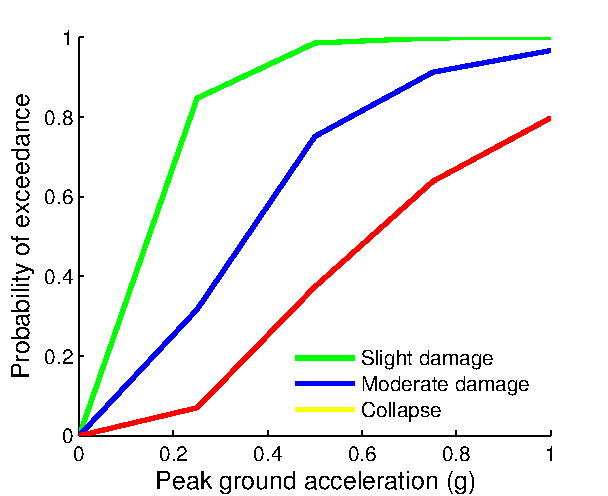
\includegraphics[width=8cm,height=6cm]{./figures/risk/DisFragilityModel.pdf}
\caption{Graphical representation of a discrete fragility model.}
\label{fig:fragModelDiscrete}
\end{figure}

Similarly to what has been described for the \glspl{vulnerability model}, the NRML schema for this input also has some attributes that are common to all of the \glspl{fragility function} comprising the model. This initial portion of the schema is depicted below:

\begin{Verbatim}[frame=single, commandchars=\\\{\}, samepage=true]
<?xml version="1.0" encoding="UTF-8"?>
<nrml xmlns:gml="http://www.opengis.net/gml"
      xmlns="http://openquake.org/xmlns/nrml/0.4">
<\textcolor{red}{<fragilityModel format="discrete">}>
    <\textcolor{green}{description} "Fragility Model for RC" <\textcolor{green}{/description}>
    <\textcolor{green}{limitStates} 
        slight damage
        moderate damage
        collapse     
    <\textcolor{green}{/limitStates}>
    ...
\end{Verbatim}

\begin{itemize}
\item  \Verb+description+: represents an attribute that can be used to include  some information about the \gls{fragility model}, for example, what building typologies are being covered or the source of the \gls{fragility model};
\item  \Verb+limitStates+: this field is used to define the number and nomenclature of each limit state. Despite the fact that three limit states are being employed in this example, it is possible to use any number of states, as long as a fragility curve is always defined for each limit state. 
\end{itemize}

\begin{Verbatim}[frame=single, commandchars=\\\{\}, samepage=true]
    ...
    <\textcolor{green}{ffs noDamageLimit= 0.05}> 
        <\textcolor{blue}{taxonomy} RC <\textcolor{blue}{/taxonomy}>
        <\textcolor{blue}{IML} IMT="PGA" imlUnit="g"> 0.0 0.25 0.50 0.75 1.00 <\textcolor{blue}{/IML}>

        <\textcolor{blue}{ffd} ls="slight damage">
            <\textcolor{magenta}{poes}> 0.0 0.85 0.98 0.99 1.00 < \textcolor{magenta}{/poes}>
        <\textcolor{blue}{/ffd}
        <\textcolor{blue}{ffd} ls="moderate damage">
            <\textcolor{magenta}{poes}> 0.0 0.32 0.75 0.91 0.97 < \textcolor{magenta}{/poes}>
        <\textcolor{blue}{/ffd}
        <\textcolor{blue}{ffd} ls="collapse">
            <\textcolor{magenta}{poes}> 0.0 0.07 0.37 0.64 0.80 < \textcolor{magenta}{/poes}>
        <\textcolor{blue}{/ffd}
    <\textcolor{green}{/ffs}>
<\textcolor{red}{/fragilityModel}>
</nrml>
\end{Verbatim}

For each building typology, a set of limit state curves need to be stored within the field \Verb+ffs+ (fragility function set). The following attributes are currently being employed to define this input:

\begin{itemize}
\item  \Verb+noDamageLimit+: this attribute defines the intensity measure level below which the probability of exceedance for all curves is zero;
\item  \Verb+taxonomy+: a unique key that is used to relate each \gls{fragility function} with the relevant \glspl{asset} in the \gls{exposure model};
\item  \Verb+IML+: this attribute serves the purposes of defining the list of intensity measure levels for which the limit state curves are defined. In addition, it is also necessary to define the intensity measure type (\Verb+IMT+) being used and the respective units (\Verb+imlUnit+);
\item  \Verb+ffd+: this field (fragility function discrete) is used to define the probabilities of exceedance (\Verb+poes+) of each limit state curve. It is also necessary to include which limit state is being defined in the attribute \Verb+ls+.
\end{itemize}

As previously mentioned, the user may choose to define the \glspl{fragility function} in a continuous manner, through the use of cumulative lognormal functions. In Figure \ref{fig:fragModelContinuous}, a continuous fragility model is presented.

\begin{figure}[ht]
\centering
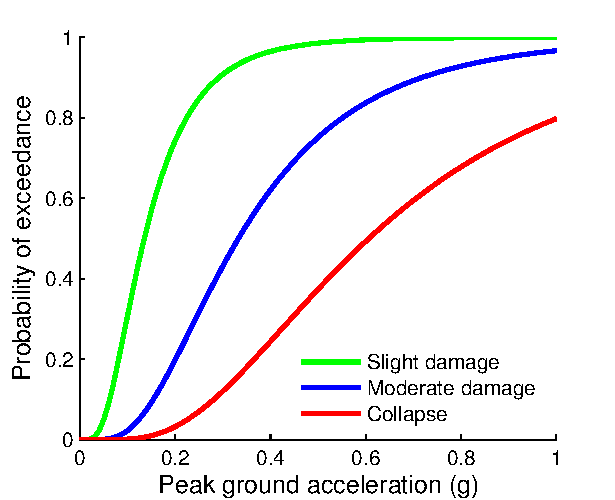
\includegraphics[width=8cm,height=6cm]{./figures/risk/ConFragilityModel.pdf}
\caption{Graphical representation of a continuous fragility model.}
\label{fig:fragModelContinuous}
\end{figure}

The NRML schema to store these functions has an initial structure similar to that described for the discrete \glspl{fragility model}. Then, the continuous limit state curves are stored as illustrated below:

\begin{Verbatim}[frame=single, commandchars=\\\{\}, samepage=true]
    ...  
    <\textcolor{green}{ffs noDamageLimit= 0.05}> 
        <\textcolor{blue}{taxonomy} RC <\textcolor{blue}{/taxonomy}>
        <\textcolor{blue}{IML} IMT="PGA" minIML="0.0" maxIML="1.0" imlUnit="g" ><\textcolor{blue}{/IML}>
        <\textcolor{blue}{ffd} ls="slight damage">
            <params \textcolor{magenta}{mean}="0.16" \textcolor{magenta}{stddev}="0.11" />
        <\textcolor{blue}{/ffd}
        <\textcolor{blue}{ffd} ls="moderate damage">
            <params \textcolor{magenta}{mean}="0.40" \textcolor{magenta}{stddev}="0.26" />
        <\textcolor{blue}{/ffd}
        <\textcolor{blue}{ffd} ls="collapse">
            <params \textcolor{magenta}{mean}="0.73" \textcolor{magenta}{stddev}="0.48" />
        <\textcolor{blue}{/ffd}      
    <\textcolor{green}{/ffs}> 
<\textcolor{red}{/fragilityModel}>
</nrml>        
\end{Verbatim}

Again, the set of limit state curves for each building typology needs to be stored within the field \Verb+ffs+ (fragility function set), through the definition of the following attributes:

\begin{itemize}
\item  \Verb+noDamageLimit+: this attribute defines the intensity measure level below which the probability of exceedance for all curves is zero;
\item  \Verb+type+: this parameter defines the type of probabilistic distribution being used to define the limit state curves. Currently the engine only supports lognormal distributions, however, the capability of considering other types of distributions (e.g. normal, exponential) will be developed in the future;
\item  \Verb+taxonomy+: a unique key that is used to relate each \gls{fragility function} with the relevant \glspl{asset} in the \gls{exposure model};  
\item  \Verb+IML+: in this field, the intensity measure type (\Verb+IMT+) and associated units (\Verb+imlUnit+) for the limit state curves is defined, along with the minimum (\Verb+minIML+) and maximum (\Verb+maxIML+) intensity measure levels enclosing the range of applicability of the set of fragility functions;
\item  \Verb+ffc+: this field (fragility function continuous) is used to define the mean (\Verb+mean+) and standard deviation (\Verb+stddev+) of the cumulative lognormal function. In addition, the limit state for the curve being defined needs to be specified in the attribute \Verb+ls+.
\end{itemize}

\subsection{Configuration file}
The configuration file (or job.ini file) represents the location where the paths to the input files, the parameters controlling the risk calculations and the type of outputs are defined. Some initial parameters common to all the risk calculators are presented below. The remaining parameters that are specific to each risk calculator are discussed in subsequent sections. For additional information about how each parameter is being used within the methodologies implemented in the oq-engine, users advised to consult the OpenQuake Engine Book (Risk). 

\begin{Verbatim}[frame=single, commandchars=\\\{\}, samepage=true]
[general]
description = Scenario Risk Nepal
calculation_mode = scenario

exposure_file = exposure_model.xml
region_constraint = 78.0 31.5,89.5 31.5,89.5 25.5,78 25.5
maximum_distance = 10
...
\end{Verbatim}

\begin{itemize}
\item  \Verb+description+: a parameter that can be used to include some information about the type of calculations that are going to be performed;
\item  \Verb+calculation_mode+: this parameter sets the type of calculations. The key word for each risk calculator is described in the following sections;
\item  \Verb+exposure_file+: this parameter is used to specify the path to the \gls{exposure model} file;
\item  \Verb+region_constraint+: this field is used to define the polygon enclosing the region of interest. Assets outside of this region will not be considered in the risk calculations. This region is defined using pairs of coordinates (longitude and latitude in decimal degrees) that indicate the vertexes of the polygon;
\item  \Verb+maximum_distance+: this parameter indicates the maximum allowable distance between an \gls{asset} and the closest hazard input. If no hazard input is found within this distance, the \gls{asset} is skipped and a message is provided mentioning the id of the asset that is affected by this issue. If this parameter is not provided, the OpenQuake-Engine assumes the maximum allowable distance as 5 km.
\end{itemize}

Depending on the type of calculations, other parameters besides the aforementioned ones need to be provided, as will be described in the following sections.

\subsubsection{Scenario Risk Calculator}
In order to run this calculator, the parameter \Verb+calculation_mode+ needs to be set to \Verb+scenario+. The remaining parameters are illustrated bellow.

\begin{Verbatim}[frame=single, commandchars=\\\{\}, samepage=true]
...
structural_vulnerability_file = struct_vul_model.xml
nonstructural_vulnerability_file = nonstruct_vul_model.xml
contents_vulnerability_file = cont_vul_model.xml
business_interruption_vulnerability_file = bus_int_vul_model.xml
occupants_vulnerability_file = occ_vul_model.xml

asset_correlation = 0.7
master_seed = 3
insured_losses = true
\end{Verbatim}

\begin{itemize}
\item  \Verb+structural_vulnerability_file+: this parameter is used to specify the path to the structural \gls{vulnerability model} file;
\item  \Verb+nonstructural_vulnerability_file+: this parameter is used to specify the path to the non-structural\gls{vulnerability model} file;
\item  \Verb+contents_vulnerability_file +: this parameter is used to specify the path to the contents \gls{vulnerability model} file;
\item  \Verb+business_interruption_vulnerability_file +: this parameter is used to specify the path to the business interruption \gls{vulnerability model} file;
\item  \Verb+vulnerability_file+: this parameter is used to specify the path to the occupants \gls{vulnerability model} file;
\item \texttt{asset\_cor\-re\-la\-tion} if the uncertainty in the loss ratios has been defined within the \gls{vulnerability model}, users can specify a coefficient of correlation that will be used in the Monte Carlo sampling process of the loss ratios, between the assets that share the same \gls{taxonomy}. If the \texttt{asset\_cor\-re\-la\-tion} is set to one, the loss ratio residuals will be perfectly correlated. On the other hand, if this parameter is set to zero, the loss ratios will be sampled independently. Any value between zero and one will lead to increasing levels of correlation. If this parameter is not defined, the OpenQuake engine assumes no correlation in the vulnerability;
\item  \Verb+master_seed+: this parameter is used to control the random generator in the loss ratio sampling process. This way, if the same \Verb+master_seed+ is defined at each calculation run, the same random loss ratios will be generated, thus allowing replicability of the results;
\item  \Verb+insured_losses+: this parameter is used to define if insured losses should be calculated (\Verb+true ) or not (\Verb+false+).
\end{itemize}

\subsubsection{Scenario Damage Calculator}
For this calculator, the parameter \Verb+calculation_mode+ needs to be defined as \Verb+scenario_damage+. There is only one parameter specific to this calculator, which is the \gls{fragility model} file path, as presented below.

\begin{Verbatim}[frame=single, commandchars=\\\{\}, samepage=true]
...
fragility_file = fragility_model.xml
\end{Verbatim}

\begin{itemize}
\item  \Verb+fragility_file+: a parameter used to define the path to the \gls{fragility model} file.
\end{itemize}

\subsubsection{Probabilistic Event-based Risk Calculator}
The parameter \Verb+calculation_mode+ needs to be set to \Verb+event_based+ in order to use this calculator. Similarly to that described for the Scenario Risk Calculator, a Monte Carlo sampling process is also employed within this module to take into account the loss ratio uncertainty. Hence, the parameters \Verb+asset_correlation+ and \Verb+master_seed+ need to be defined as previously described. This calculator is also capable of estimating insured losses and therefore, the \Verb+insured_losses+ attribute should be established as well.
For what concerns the loss disaggregation, the Probabilistic Event-based Risk Calculator can disaggregate the losses based on magnitude/distance and location (longitude/latitude) of the events. In order to do so, it is necessary to define the bin width of each of these parameters, as illustrated in the following example.

 The remaining parameters are presented below.

\begin{Verbatim}[frame=single, commandchars=\\\{\}, samepage=true]
...
structural_vulnerability_file = struct_vul_model.xml
nonstructural_vulnerability_file = nonstruct_vul_model.xml
contents_vulnerability_file = cont_vul_model.xml
business_interruption_vulnerability_file = bus_int_vul_model.xml
occupants_vulnerability_file = occ_vul_model.xml

asset_correlation = 0.7
master_seed = 3
insured_losses = true

sites_disagg = 85.07917, 27.4625
mag_bin_width = 0.5
distance_bin_width = 20
coordinate_bin_width = 0.5

loss_curve_resolution = 20
conditional_loss_poes = 0.01, 0.05, 0.1
\end{Verbatim}

\begin{itemize}
\item \Verb+loss_curve_resolution+: since this calculator uses an event\--based ap\-proach, a large number of levels of loss (and associated probabilities of exceedance) is computed (one per event) for each asset. The oq-risklib will use this large set of results to extrapolate a loss curve, whose number of points are controlled by this parameter. By default, the OpenQuake engine assumes the \Verb+loss_curve_resolution+ equal to 20;
\item  \Verb+conditional_loss_poes+: this parameter is used to define the probabilities of exceedance at which loss maps are to be produced;
\item  \Verb+sites_disagg+: list of locations (pairs of longitude and latitude) where the loss disaggregation should be carried out. Notice that in order to perform the loss disaggregation, assets needs to exist at those locations;
\item  \Verb+mag_bin_width+: this parameter specifies the with of the magnitude bins (in Mw);
\item  \Verb+distance_bin_width+: this parameter specifies the with of the distance bins (in km);
\item  \Verb+coordinate_bin_width+: this parameter specifies the with of the coordinates bins (in decimal degrees);
\end{itemize}

The definition of the parameters for the loss disaggregation follow the same rules established for the seismic hazard disaggregation described in section (TO BE INCLUDED).

\subsubsection{Classical PSHA-based Risk Calculator}
In order to run this calculator, the parameter \Verb+calculation_mode+ needs to be set to \Verb+classical+. With this calculator it is also possible to extract loss maps, so the parameter \Verb+conditional_loss_poes+ needs to be defined as explained in the previous sub-section. The remaining parameter is illustrated below.
\begin{Verbatim}[frame=single, commandchars=\\\{\}, samepage=true]
...
structural_vulnerability_file = struct_vul_model.xml
nonstructural_vulnerability_file = nonstruct_vul_model.xml
contents_vulnerability_file = cont_vul_model.xml
business_interruption_vulnerability_file = bus_int_vul_model.xml
occupants_vulnerability_file = occ_vul_model.xml

lrem_stpdf_per_interval = 2
conditional_loss_poes = 0.01, 0.05, 0.1
\end{Verbatim}

\begin{itemize}
\item  \Verb+lrem_stpdf_per_interval+: this parameter controls the number of intermediate values between consecutive loss ratios (as defined in the \gls{vulnerability model}) that are considered in the risk calculations. A larger number of loss ratios than those defined in each \gls{vulnerability function} should be considered, in order to better account for the uncertainty in the loss ratio distribution. If this parameter is not defined in the configuration file, the OpenQuake engine assumes the \Verb+lrem_stpdf_per_interval+ to be equal to 5. More details are provided in the OpenQuake Engine Book (Risk).  
\end{itemize}

\subsubsection{Retrofitting Benefit/Cost Ratio Calculator}
As previously explained, this calculator uses loss exceedance curves which can be calculated using the Classical PSHA-based Risk or the Probabilistic Event-based Risk calculators. Therefore, depending on which calculator a user chooses to employ, the configuration file will be different. If the Classical PSHA-based Risk calculator is employed, then the \Verb+calculation_mode+ should be set to \texttt{clas\-si\-cal\_bcr} and the calculator-specific part of the configuration file should be defined as presented below.

\begin{Verbatim}[frame=single, commandchars=\\\{\}, samepage=true]
...
structural_vulnerability_file = struct_vul_model.xml
vulnerability_retrofitted_file = retrof_vul_model.xml

lrem_stpdf_per_interval = 2

interest_rate= 0.005
asset_life_expectancy = 50
\end{Verbatim}

\begin{itemize}
\item  \Verb+vulnerability_retrofitted_file+: this parameter is used to specify the path to the \gls{vulnerability model} file containing the \glspl{vulnerability function} for the retrofitted assets;  
\item  \Verb+interest_rate+: this parameter represents the interest rate and it serves the purposes of taking into account the variation of building value throughout time;
\item  \Verb+asset_life_expectancy+: this variable defines the life expectancy, or design life, of the assets.
\end{itemize}

Alternatively, if a user decides to employ the Probabilistic Event-based Risk calculator for the calculation of the loss curves, then the \Verb+calculation_mode+ should be set to \Verb+event_based_bcr+ and the remaining portion of the configuration file should be defined as follows.

\begin{Verbatim}[frame=single, commandchars=\\\{\}, samepage=true]
...
vulnerability_file = vulnerability_model.xml
vulnerability_retrofitted_file = vulnerability_model_retrof.xml
asset_correlation = 0.7
master_seed = 3

loss_curve_resolution = 20

interest_rate= 0.005
asset_life_expectancy = 50
\end{Verbatim}